%!TEX root = ../dynamics.tex
\section{Market Analysis}
\label{sec:market}



\begin{figure}[htbp]
	\centering
		
\includegraphics[width=0.5\textwidth]{figures/scattermatrix}
	\caption{Supply and demand relationship}
	\label{fig:scatter_matrix}
\end{figure}
In Figure\ref{fig:scatter_matrix} we show the relationship between demand: number of new HITs posted
and supply: work completed.


\begin{figure}[htbp]
	\centering
		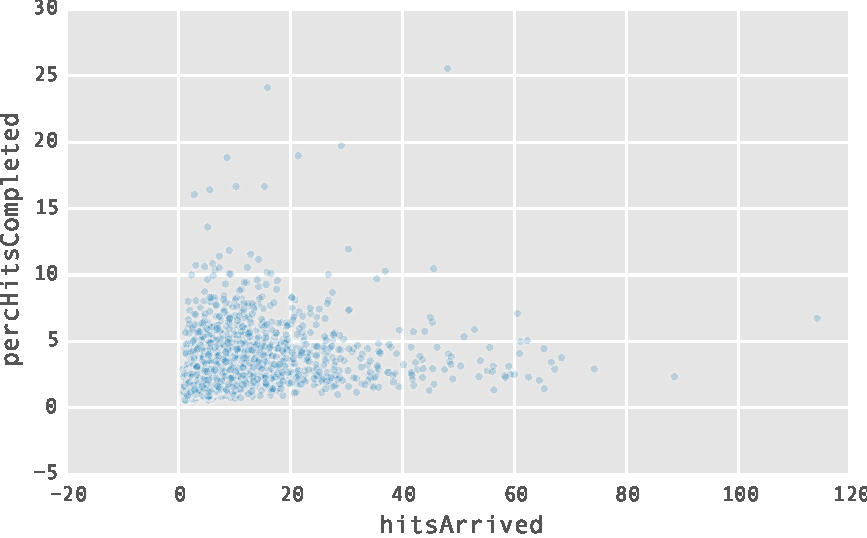
\includegraphics[width=0.5\textwidth]{figures/percHitsCompleted}
	\caption{The effect of new arrived HITs on the work provided supplied.}
	\label{fig:perc_hits_completed}
\end{figure}
The results detailed in Figure\ref{fig:perc_hits_completed} indicate that as more HITs arrive, a *higher* *percentage* of the available work
gets done. This clearly indicates that the arrival of new work also attracts new workers
in the market, who also seem to spillover to other tasks

\begin{figure}[htbp]
	\centering
		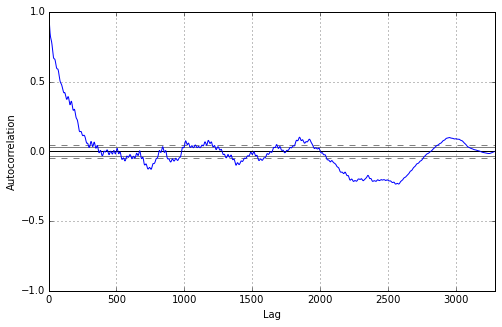
\includegraphics[width=0.5\textwidth]{figures/autocorrelation_plot}
	\caption{Autocorrelation  1}
	\label{fig:autocorrelation1}
\end{figure}
(Panos) It seems that there is significant memory for the market, as the autocorrelation of the 
HITS available (as reported by Amazon) lasts for approximately 7-10 days

\begin{figure}[htbp]
	\centering
		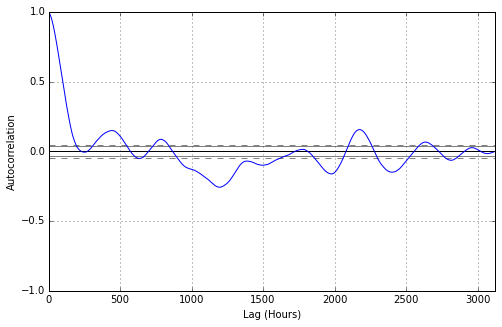
\includegraphics[width=0.5\textwidth]{figures/autocorrelation2}
	\caption{Autocorrelation 2}
	\label{fig:autocorrelation2}
\end{figure}

@Panos: The plot shows a strong weekly periodicity